\documentclass[12pt]{article}
\usepackage[utf8]{inputenc}
\usepackage{graphicx}
\usepackage{setspace}
\graphicspath{ {images/} }
\usepackage{lipsum}
\usepackage{makecell}
%%%%%%%%%%%%%%%%%%%%%%%%%%%%%%%%%%%%%%%%%%%%%%%%%%%%%%%%%%%%%%%%%%%%%%%%%%%%%%%%%%%%%%%%%%%%%%%%%%%%%%%%%
%%%%%%%%%%%%%%%% HEADER PART %%%%%%%%%%%%%%%%%%%%%%%%%%%%%%%%%%%%%%%%%%%%%%%%%%%%%%%%%%%%%%%%%%%%%%%%%%%%
\usepackage[a4paper,right=1.0in,top=1in,bottom=1in,left = 1.0in,width=150mm,bindingoffset=6mm]{geometry}
\begin{document}
	% !TEX root = ../thesis-example.tex
%
% ------------------------------------  --> cover title page
\begin{titlepage}
%	\pdfbookmark[0]{Cover}{Cover}
	\begin{center}
	\hfill
	
   
	\rule[5pt]{\textwidth}{1.0pt} \par
{\Huge \textbf{DevOps Tools Training at Dell EMC} \par}
\rule[5pt]{\textwidth}{1.0pt} \par

	\vspace*{1cm}
	{\large \fontfamily{ppl}\centering\textit{An Industrial Internship Training Report}\par \vspace*{1cm}
	\textit{submited to}\par
		{\Large JSS Science \& Technology University} \par  
		{
\includegraphics[width=0.4\textwidth]{logo.jpg}} \par
		{\textit{for the fulfillment of the requirements for the degree of \\ Master of Technology}\par in \par\textit{Data Science} \par	\vspace*{1cm}
			\vspace*{2cm}
			\textit{submited by} \hfill \textit{Mentor}\par
			\vspace*{0.5cm}
			\textit{Kishore G R} \hfill \textit{Gourishankar Mohapatra,}\par
			\textit{USN - 01JST19PDS005} \hfill \textit{Manager, Software Engineer,}\par
			\hfill \textit{Dell EMC, Bagmane Tech Park, Bengaluru.}\par
            \hfill \textit{Gourishankar\_Mohapatra@Dell.com}
	    \vfill
	    \large\fontfamily{ppl} {Department of Information Science \& Engineering}\par
		\small \fontfamily{ppl}{JSS Science \& Technology University (SJCE), Mysuru}} 

	\vfill
}
%	\textit{\large\Submitted by} \\
%	Version: \thesisVersion
	\end{center}
\end{titlepage}


% ------------------------------------  --> main title page
%\begin{titlepage}
%	\pdfbookmark[0]{Cover}{Cover}
%	\flushright
%	\hfill
%	\vfill
%	{\LARGE\thesisTitle \par}
%	\rule[5pt]{\textwidth}{.4pt} \par
%	{\Large\thesisName}
%	\vfill
%	\flushleft
%%	\textit{\large\thesisDate} \\
%	 Copyright \copyright \the\year \par
%	Permission is granted to copy, distribute and\slash or modify 
%	this document under the terms of the GNU 
%%	Version: \thesisVersion
%\end{titlepage}


% ------------------------------------  --> lower title back for single page layout
%\hfill
%\vfill
%{
%	\small
%	\textbf{\thesisName} \\
%%	\textit{\thesisTitle} \\
%%	Department of Information Science \& Engineering\thesisSubject, \thesisDate \\
%%	Reviewers: \thesisFirstReviewer \\
%%	Supervisors: \thesisFirstSupervisor \\[1.5em]
%%	{Department of Information Science \& Engineering} \\
%%	\textit{\thesisUniversityGroup} \\
%	\thesisUniversityDepartment \\
%	\thesisUniversityInstitute \\
%	\thesisUniversityStreetAddress \\
%	\thesisUniversityPostalCode\ \thesisUniversityCity
%}

	\begin{center}
\emph{\LARGE\textbf {Certificate}}\\[2.5cm]
\end{center}


\doublespacing
This is to certify that Mr. \textit{Kishore G R} from the M.Tech in Data Science Department of JSS Science \& Technology University, Mysuru has completed the Industrial Training under my supervision. He was trained in the field of \textit{DevOps Build Tools} from July 20, 2020 to July 16, 2021 for the academic year 2020-2021. His works is found satisfactory. 

\vspace*{4cm}

%hfill (space for signature)\par
\hfill \textit{Gourishankar Mohapatra,}\par
\hfill \textit{Dell EMC, Bagmane Tech Park, Bengaluru.}\par
\hfill \textit{Gourishankar\_Mohapatra@Dell.com}

	\newpage
	\begin{center}
\emph{\LARGE\textbf {Abstract}}\\[2.5cm]
\end{center}


\doublespacing
Agriculture plays a pivotal role in human’s life as it the only source of livestock, along with that it also provides employment opportunities and plays a major role in country’s economy, hence it is important to maintain standards in production quality. Recent advancements in technology have led to the hybridization of agriculture and machine learning methodologies thus helping in the improvement of crop quality. However it is observed from the literature survey that most of the work focuses on detection of crop damage and not on cause of damage, hence in this work an attempt is made to identify the cause of damage especially considering the case of pesticide usage. For this experiment the dataset of around 1.48 lakh samples has been used to train and predict the cause of crop damage with the help of some of the well know machine learning models. The results show that LGBM performs better than other models both in terms of classification accuracy and speed. 
\vspace*{4cm}




	\newpage
	\tableofcontents
	\newpage
	\listoftables
	\newpage
	\listoffigures
	\newpage
	\section{Introduction}
	
Agriculture is the science and a key practise of cultivation followed by humans to fulfil their daily needs. The word agriculture is combination of Latin words ‘Agri’ which means field and ‘cultura’ meaning cultivation. Agriculture plays a very important role in the rise of civilization. It enables people to produce almost everything that are considered as basic needs in everyone’s life such as, cultivating food products like wheat, barley etc., producing cotton and wool that can be used for clothing and timber which help humans to build shelters. Farming is one of the main divisions of agriculture which can be classified into two types, one is arable farming where the crops such as wheat and barley are grown and the other is pastoral farming which is more of husbandry that is, raising and taking care of animals.

Agriculture is livelihood for majority of population in India, although its contribution was low in country's economy, the improvement in farming techniques and methodology in recent years has helped in increasing its contribution to GDP in a faster rate. This is also possible due to the hybridisation of machine learning approaches with agriculture science. A well-trained ML model helps in getting more accurate results in short time when compared to traditional procedures. An automated farming setup helps in monitoring the crops, its surrounding environmental condition and triggering of appropriate action without much of human intervention, thus maintaining a suitable condition for crops which will be a very difficult task for a human to continuously monitor and track all the condition otherwise.

When it comes to arable farming they have their own set of challenges such as harmful organisms like pests, weeds or other diseases. This leads to the usage of pesticides; which are used to control pests and disease carriers, thus helping the plants to grow in a protected environment, but at the same time excess use of pesticide can affect soil fertility, can even affect health of the consumer. Hence pesticides should be used in reasonable quantities. A crop can be damaged due to other reasons as well such as flood, animal trespassing etc. Hence the conditions of crop can be classified as shown in figure 1.


\begin{figure}[hbt!]
\center
{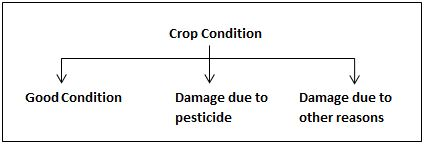
\includegraphics[scale=0.7]{cat.jpg}}
\caption{Classification of crop conditions}
\end{figure}

Here the Good condition is when the crop is healthy and the yield is good, damage due to pesticide is when the crop is damaged due to inadequate or excess use of pesticides and the last is when the crop is damaged due to unidentified or natural causes. This work discusses the classification of crop into above mentioned categories with the help of machine learning approaches that are mentioned in section 1.2 of this report.

	\subsection{Related Works }
	An extensive survey has been made to understand the existing machine learning methodologies and techniques that are being used in the field of agriculture.
	
When it comes to image or computer vision in agriculture, [1][10][11][13] concludes that CNN performs very well  and detects maximum number of diseases with high accuracy. Whereas [12] uses a standard GoogleNet CNN model for the same. [2] Performs a comprehensive survey and suggests specific statistical ML technique for specific purpose by analysing each technique in machine vision systems. For yield prediction, an extensive investigation done by [3] shows that CNN is the most widely deep learning algorithm followed by Long-Short Term Memory (LSTM) and Deep Neural Networks (DNN) models. In [5] researches conducted in the last 15 years are discussed and they conclude that the targeted development of hybrid systems formed by combining machine learning and signal processing will act as a cost effective solution for a good crop and helps in decision making. The authors in [21] shows that adding weather and non-weather predictor variables to Normalized Difference Vegetation Indices (NDVI) with ANN as model gives the better yield predictions. [22] Uses random forest for crop yield prediction with climate and biophysical related values being the variables. As there is high chance for a crop to get a disease, it is important to identify them immediately for a good yield and for that, some of the works gives us valuable insight such as [7], where the author performs classification of images to identify the Scorch Diseases in sugar cane leaf by using k-Means clustering for segmentation and k-Nearest Neighbour for classification, with an accuracy of 95\%. Similarly [8] performs classification using k-NN with an accuracy of 76.59\%, but uses Otsu segmentation method and the experiment is performed on paddy leaves to identify blast and brown spot diseases. The authors in [9] proposed a method where the plant leaf disease is detected with the help of texture features obtained by colour co-occurrence matrix, and SVM is used for classification and this model performs with an accuracy of 94\%.

When it comes to using IoT in agriculture, [15] discusses how the combination of the Internet of Things (IoT) and machine learning can be used in the field of agriculture leading to smart farming model to increase the productivity. [16] proposed a neural network model that can be used as an alternative method to simulate the groundwater level changes especially in regions where subsurface properties are unknown. [17] used ML models such as random forest and support vector machine (SVM) to assess the land suitability for rain-fed crops in agricultural land, whereas [19] used k-nearest-neighbour and boosted perceptron algorithms to assess the soil dryness in agricultural land which performed with an accuracy of around 92\%.  [4] presents the role of ML models in agriculture supply chain, and provides guidelines for the improved sustainability and productivity.

We can observe from the survey that there are very less discussions about pesticide and the cause behind the crop damage. Hence in this work an attempt has been made to give some insight on that area i.e., crop damage in terms of pesticide usage.


	\subsection{Prediction models}
In this section, the classification models used in the experiment are discussed. Considering the fundamental details of the data being used for analysis, the following supervised learning models are selected.
	
\subsubsection{k-Nearest Neighbour  (k-NN)} 
K-NN is one of the well-known lazy learning algorithms; the k in k-NN is the number of nearest neighbours to be considered during voting process. Hence the first step of this algorithm is to set k value, and then comes calculating the distance between test data and training samples. Once the distances are computed get the top k closest samples in training set and return the most frequent class among them as predicted class.


\subsubsection{Naïve Bayes}
Naive bayes is a probabilistic classifier; it gives the likelihood of occurrence of an event. That is, for any given input naive bayes algorithm returns the probability of the input being classified to a specific category. So this method involves bayes theorem with class C having k possible outcomes and it is given as

\begin{equation} 
 Pr(C_k | x)= \frac{Pr(C_k).Pr(x|C_k)}{Pr(x)}                       
\end{equation}

Where $Pr(C_k|x)$ is the posterior which is the probability of sample X being classified to Kth class. However in our case Bernoulli naïve bayes is used and hence the likelihood is given as [25]

\begin{equation} 
 Pr(x | C_k)= \prod_i^n p_{ki}^{xi}(1- p_{ki})^{(1-x_i)}                 
\end{equation}

Where $p_ki$ is the probability of class $C_k$ generating the term $x_i$ .

\subsubsection{Random forest}
Random forest also known as random decision forest is one of the ensemble learning method for classification where it collects the result from a forest of decision trees for classification thus improving the performance of a model. For this it uses one of the important steps known as bagging where it randomly selects the sample from the training set and fits the tree.

	Then in order to average out the predictions following function is used,
	
\begin{equation} 
 f'= \frac{1}{B} \sum^{B}_{b=1}f_b(x')                   
\end{equation}
Where B is number of bagging, $f_b$ being the trained classification tree function and x' being the unknown sample for which the prediction is to be done.

\subsubsection{XGBoost}
XGBoost stands for Extreme Gradient Boost is one of the ensemble tree methods.  Basically in a boosting technique, the succeeding model tries to correct the errors made by previous models. A gradient boosting tries to optimize the loss function whereas XGBoost the optimization is done along with regularization factors.

\subsubsection{Light Gradient Boosting Machine (LGBM)}
LGBM is one more decision tree based high performing gradient boosting framework which is fast when compared to other gradient boosting techniques and the reason behind this is the fact that in LGBM the tree is split leaf-wise unlike other boosting algorithms where the tree is split depth wise. Hence Light GBM reduces more loss while growing the same leaf than the ones that grow level wise thus resulting in high classification accuracy over other existing boosting algorithms.

\subsubsection{Support Vector Machine (SVM)}
SVM is one of the supervised learning algorithms, which can also be analysed mathematically.  It has a unique ability to handle the non-linearity in the input space linearly in a corresponding high dimensional feature space. [26]
	SVM basically tries to fit a hyper plane such that, 
\begin{equation} 
 (w*x)+b=0 \in R^N, b \in R 
\end{equation}

Where the marginal distance between the plane and the support vectors (SV) of two classes will be maximal, thus separating the samples effectively. In some cases in order to fit hyper plane a kernel function will be used due to the non-linearity in the input data. These kernel functions help in mapping into other dot product space thus letting the machine to fit a hyper plane. In this experiment radial basis function (RBF) kernel is used.  Where the RBF kernel on two samples x and x’ is given as,

\begin{equation} 
 K(x,x')= \exp(-\frac{||x-x'||^2 }{2\sigma^2})  
\end{equation}
	\subsection{problem definition}
The goal of this project is to classify the crops into 3 categories indicating whether the crop is Good, damaged due to pesticide or by other reasons using machine learning models and compare the performance of each model in predicting the cause of crop damage.  
	\clearpage
	
	\section{Proposed method}
	
\begin{figure}[hbt!]
\center
{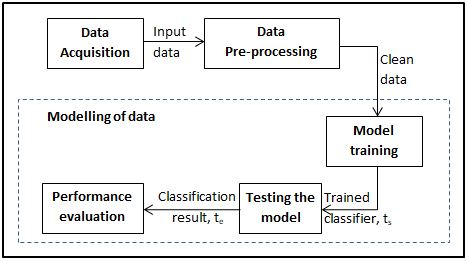
\includegraphics[scale=1]{method.jpg}}
\caption{Work-flow of proposed method}
\end{figure}	
	The above figure shows the generic flow of the proposed methodology where the first step is data acquisition, here the crop data on which the experiment needs to be performed is collected. Then the collected raw data undergoes pre-processing, where the null values are handled either by dropping the rows or by filling them manually and other actions such as dimensionality reduction and label encoding are performed. Now that the data is clean, it is ready to be fed into machine learning model in this case it is classification model.	
	
	The emphasised section of the block diagram i.e., model training, model testing and performance evaluation is generic where the classification model acts as a varying component in the setup.
	
	In order to calculate the time T taken by a model to classify a sample for a particular category, two time values i.e., the start time ts and end time te are considered , now $t_e - t_s$   will give the total time T taken for classification, more details about this are discussed in the next section.

\subsection{Dataset}
	Since the aim of this experiment is to identify the cause of crop damage, a suitable dataset is collected which contains both categorical and numerical data with the sample size of around 148k and about 11 features comprising some of the crop related details such as the type of crop, soil, the pesticides usage counts and the season.

\subsection{Time complexity}
For a machine learning algorithm along with accuracy, time complexity also plays an important role; Table 1 gives the time complexity of each model that are considered in our experiment.

The following table tabulates the theoretical time complexity of both training and testing phase of the classification models.


\begin{table}[ht]
\centering

\caption{Theoretical Time Complexity of Models}
\begin{tabular}{|c|c|c|}
\hline 
Model & Time complexity & Description \\ 
\hline 
LBGM & \makecell{O(nm) for histogram building \\
 O(bm) for split finding}
 & \makecell{n = samples, m= features\\
b=bins}
 \\ 
\hline 
XGBoost & \makecell{O(tdxlogn) to train\\
O(td) to predict new sample}
 & \makecell{t = number of trees\\
d = height of the trees and \\
x = number of non-missing\\ entries in the training data.}
 \\ 
\hline 
Naïve Bayes & \makecell{O(nm) to train. \\
O(mc), to predict new sample}
 & \makecell{n = samples, m= features\\
c = number of classes.}
 \\ 
\hline 
SVM & \makecell{Between $O(n^2m$) and $O(n^3m)$ \\depending on hyper-parameters.\\
O(vm), to predict new sample }
 & \makecell{n = samples, m= features\\
v = number of support \\vectors obtained by training}
 \\ 
\hline 
Random Forest &\makecell{ O(tunlogn), to train.\\
O(tlogn), to test new sample}
 & \makecell{n = samples,\\ t = number of trees and\\ u = number of features \\considered for splitting} \\ 
\hline 
k-NN & \makecell{O(1) for training\\
O(k*n*m) to test new sample}
 & \makecell{n = samples, m= features\\
k = number of neighbours}
 \\ 
\hline 
\end{tabular} 
\label{tab:caption}
\end{table}


Whereas Table 2 presents the practical time complexity, obtained by classification model for classifying a sample from each category that are considered in the experiment. 


\begin{table}[ht]
\centering

\caption{Practical time taken by Models}
\begin{tabular}{|c|c|c|c|}
\hline 
Model & Alive & Damage Due To other Reasons  & Damage Due To pesticide  \\ 
\hline 
LGBM & 0 & 0 & 0.015625 \\ 
\hline 
Random Forest & 0.018988 & 0.018989 & 0.018988 \\ 
\hline 
SVM & 0 & 0 & 0.015626 \\ 
\hline 
Naive Bayes & 0.015621 & 0 & 0 \\ 
\hline 
kNN & 0.004999 & 0.003996 & 0.002999 \\ 
\hline 
\end{tabular} 
\label{tab:caption}
\end{table}

The time values shown in following table is the time taken by a model for testing a sample from each category and not for training the sample. Also these are not standard time for classification by the above considered models, as the classification time depends on many aspects such as, configuration of the system on which the experiment is being done, the implementation methodology and its setup. However, the intention of this table is to show the time difference between the models (executed in a system with reasonable configuration).

 It can be seen from the above table that Random forest takes more time for classification and LGBM, naïve bayes and SVM take almost same amount of time, whereas it can also be observed how k-NN has a negligible time difference to classify a sample from each category.



\subsection{Results and discussion}
	In this section we will discuss the implementation results of the proposed approach.  
	
	As the aim of this experiment is to classify the crop into 3 categories, it is designed in such a way that it helps us to identify the model that can effectively handle all 3 categories with good classification accuracy.  Table 3 shows the classification performance of each model.
	
\begin{table}[ht]
\centering

\caption{Model performance}
\begin{tabular}{|c|c|c|c|c|}
\hline 
Model & Accuracy score & F1 score & Recall score & Precision score \\ 
\hline 
LBGM & 0.977155 & 0.875336 & 0.82776 & 0.964732 \\ 
\hline 
Random Forest & 0.835472 & 0.303454 & 0.333333 & 0.278491 \\ 
\hline 
XGBoost & 0.969531 & 0.812949 & 0.76614 & 0.941907 \\ 
\hline 
SVM & 0.835472 & 0.303454 & 0.333333 & 0.278491  \\ 
\hline 
Naive Bayes & 0.715479 & 0.448859 &	0.555625 & 0.442842 \\ 
\hline 
k-NN & 0.914754	& 0.658742	& 0.597566 & 0.843498 \\ 
\hline 
\end{tabular} 
\label{tab:caption}
\end{table}

 It can be observed from above table that Naïve bayes perform poorly when compared to other models, but it can also be seen that the $F_1-score$ of Random Forest (RF) and SVM is low when compared to naïve bayes and yet they both perform better with a classification accuracy of around 83\%. This particular comparison helps us to understand that using $F_1-score$ as a metric of performance to compare two models is wrong. The model with high $F_1-score$ doesn't mean that particular model is better than the one with lower $F_1-score$. 
 
The experiment also shows that k-NN, random forest and LGBM perform very well and they have high precision and low recall, showing that they classify so well that the models have around 84\%, 94\% and 96\% of true positive values respectively. But LGBM is the clear winner with a classification accuracy of around 97.7\%.


\clearpage

	\section{Conclusion}
	\subsection{Briefly summarize the work done}
	In this work, an attempt is made to classify the crop into three categories i.e., good crop, crop damage due to pesticides and crop damage due to other reasons. The main objective behind this work is to identify the cause behind the crop damage, this work plays a major role in decision making, like whether the pesticide doses are to be varied or the need for other precaution for a crop to grow in a protected environment. It can be observed from the experiment that all the classification models that are considered perform very well. However LGBM leads by giving an accuracy of around 97\% with minimum computational time.
	
The experiment also helps to emphasize the fact that a good classification result can be obtained without using any complex models such as neural networks. 
  
	\subsection{Future Enhancement}
	In future work, more importance is given towards the improvement of classification performance and to try and consider some of the fundamental sections of agriculture that are neglected in existing methodologies in the analysis to identify their contribution for a good yield of crop with the help of machine learning models.
\clearpage	
	\addcontentsline{toc}{section}{References}
	
	\begin{thebibliography}{9}
\bibitem{bib1}	U. Shruthi, V. Nagaveni and B. K. Raghavendra, "A Review on Machine Learning Classification Techniques for Plant Disease Detection," 2019 5th International Conference on Advanced Computing \& Communication Systems (ICACCS), Coimbatore, India, 2019, pp. 281-284, doi: 10.1109/ICACCS.2019.8728415.
\bibitem{bib2}	Tanzeel U. Rehman, Md. Sultan Mahmud, Young K. Chang, Jian Jin, Jaemyung Shin,Current and future applications of statistical machine learning algorithms for agricultural machine vision systems,Computers and Electronics in Agriculture,Volume 156,2019,Pages 585-605.
\bibitem{bib3}	Thomas van Klompenburg, Ayalew Kassahun, Cagatay Catal,Crop yield prediction using machine learning: A systematic literature review,Computers and Electronics in Agriculture,Volume177,2020.
\bibitem{bib4}	Rohit Sharma, Sachin S. Kamble, Angappa Gunasekaran, Vikas Kumar, Anil Kumar,A systematic literature review on machine learning applications for sustainable agriculture supply chain performance,Computers \& Operations Research,Volume 119,2020.
\bibitem{bib5}	Anna Chlingaryan, Salah Sukkarieh, Brett Whelan,Machine learning approaches for crop yield prediction and nitrogen status estimation in precision agriculture: A review,Computers and Electronics in Agriculture,Volume 151,2018,Pages 61-69.
\bibitem{bib6}	Diego Inácio Patrício, Rafael Rieder,Computer vision and artificial intelligence in precision agriculture for grain crops: A systematic review,Computers and Electronics in Agriculture,Volume 153,2018,Pages 69-81.
\bibitem{bib7}	 Umapathy Eaganathan, Jothi Sophia, Vinukumar Lackose and Feroze Jacob Benjamin, "Identification of Sugarcane Leaf Scorch Disease using K-means Clustering Segmentation and KNN based Classification", International Journal of Advances in Computer Science and Technology (IJACST), vol. 3, no. 12, pp. 11-16, 2014.
\bibitem{bib8}	M. Suresha, K. N. Shreekanth and B. V. Thirumalesh, "Recognition of diseases in paddy leaves using knn classifier," 2017 2nd International Conference for Convergence in Technology (I2CT), Mumbai, 2017, pp. 663-666.
\bibitem{bib9}	S. Arivazhagan, R. Newlin Shebiah, S. Ananthi and S. Vishnu Varthini, "Detection of unhealthy region of plant leaves and classification of plant leaf diseases using texture features", Agric Eng Int: CIGR Journal, vol. 15, no. 1, pp. 211, March 2013.
\bibitem{bib10}	JOUR, Van Hulle, Marc, Sladojevic, Srdjan, Arsenovic, Marko, Anderla, Andras, Culibrk, Dubravko, Stefanovic, Darko, 2016, 2016/06/22, Deep Neural Networks Based Recognition of Plant Diseases by Leaf Image Classification,3289801,2016,1687-5265.
\bibitem{bib11}	Konstantinos P. Ferentinos, Deep learning models for plant disease detection and diagnosis, Computers and Electronics in Agriculture, Volume 145, 2018, Pages 311-318.
\bibitem{bib12}	Jayme Garcia Arnal Barbedo, Plant disease identification from individual lesions and spots using deep learning, Biosystems Engineering, Volume 180, 2019, Pages 96-107.
\bibitem{bib13}	 M. Francis and C. Deisy, "Disease Detection and Classification in Agricultural Plants Using Convolutional Neural Networks — A Visual Understanding," 2019 6th International Conference on Signal Processing and Integrated Networks (SPIN), Noida, India, 2019, pp. 1063-1068.
\bibitem{bib14}	Agarwal M., Sinha A., Gupta S.K., Mishra D., Mishra R. (2020) Potato Crop Disease Classification Using Convolutional Neural Network. Smart Systems and IoT: Innovations in Computing. Smart Innovation, Systems and Technologies, vol 141. Springer.
\bibitem{bib15}	Balducci, Fabrizio; Impedovo, Donato; Pirlo, Giuseppe. 2018. "Machine Learning Applications on Agricultural Datasets for Smart Farm Enhancement." Machines 6, no. 3: 38. issue of 2016, MDPI journals
\bibitem{bib16}	Sahoo, S., Russo, T. A., Elliott, J., and Foster, I. (2017), Machine learning algorithms for modeling groundwater level changes in agricultural regions of the U.S., Water Resour. Res., 53, 3878– 3895.
\bibitem{bib17}	 Taghizadeh-Mehrjardi, R.; Nabiollahi, K.; Rasoli, L.; Kerry, R.; Scholten, T. Land Suitability Assessment and Agricultural Production Sustainability Using Machine Learning Models. Agronomy 2020, 10, 573. MDPI journals
\bibitem{bib18}	Abderrachid Hamrani, Abdolhamid Akbarzadeh, Chandra A. Madramootoo, Machine learning for predicting greenhouse gas emissions from agricultural soils, Science of The Total Environment, Volume 741, 2020.
\bibitem{bib19}	Evan J. Coopersmith, Barbara S. Minsker, Craig E. Wenzel, Brian J. Gilmore, Machine learning assessments of soil drying for agricultural planning, Computers and Electronics in Agriculture, Volume 104, 2014, Pages 93-104.
\bibitem{bib20}	Doh, Benjamin \& Zhang, Duo \& Shen, Yue \& Hussain, Fida \& Doh, Ronky \& Ayepah, Kwaku. (2019). Automatic Citrus Fruit Disease Detection by Phenotyping Using Machine Learning. 1-5. 
\bibitem{bib21}	Chandra, A. \& Mitra, P. \& Dubey, Sunil \& Ray, Shibendu. (2019). Machine learning approach for kharif  rice yield prediction integrating multi-temporal vegetation indices and weather and non-weather variables. ISPRS - International Archives of the Photogrammetry, Remote Sensing and Spatial Information Sciences. 
\bibitem{bib22}	Jeong, Jighan \& Resop, Jonathan \& Mueller, Nathaniel \& Fleisher, David \& Yun, Kyungdahm \& Butler, Ethan \& Timlin, Dennis \& Shim, Kyo-Moon \& Gerber, James \& Reddy, Vangimalla \& Kim, Soo-Hyung. (2016). Random Forests for Global and Regional Crop Yield Predictions.
\bibitem{bib23}	Champaneri, Mayank \& Chachpara, Darpan \& Chandvidkar, Chaitanya \& Rathod, Mansing. (2020). Crop yield prediction using machine learning. International Journal of Science and Research (IJSR).
\bibitem{bib24}	D. Wettschereck and D. Thomas G., “Locally adaptive nearest neighbour algorithms,” Adv. Neural Inf. Process. Syst., pg. 184–186, 1994
\bibitem{bib25}	24.	Machine learning Naïve Bayes classifiers, CS340 (Machine learning) Fall 2007. 
\bibitem{bib26}	Marti A. Hearst (1998) Support vector machines. IEEE intelligent systems.


		

	\end{thebibliography}
	
	
\end{document}
